\chapter{Basic Data Representation}
\label{chap:basic_data_representation}

\begin{figure}[ht]
	\hfill
	\begin{minipage}{0.5\textwidth}
		\centering
		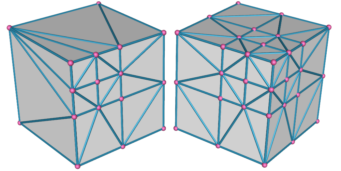
\includegraphics{VTKTextbook-48}\\
		\caption*{\texttt{Compatible tessellations.}}
	\end{minipage}
\end{figure}

\firstletter{I}n Chapter 4 we developed a pragmatic definition of the visualization process: mapping information into graphics primitives.
We saw how this mapping proceeds through one or more steps, each step transforming data from one form, or data representation, into another.
In this chapter we examine common data forms for visualization.
The goal is to familiarize you with these forms, so that you can visualize your own data using the tools and techniques provided in this text.

\section{Introduction}
To design representational schemes for data we need to know something about the data we might
encounter. We also need to keep in mind design goals, so that we can design efficient data structures
and access methods. The next two sections address these issues.

\subsection{Characterizing Visualization Data}
Since our aim is to visualize data, clearly we need to know something about the character of the
data. This knowledge will help us create useful data models and powerful visualization systems.

\section{Bibliographic Notes}

A variety of representation schemes have been proposed for each dataset type described here. These schemes vary depending on design goals. For example, even the simple volume representation has been implemented with other more complex schemes such as run-length encoding and octrees \cite{Bloomenthal88}. A description of more general representation schemes is available in \cite{Haber91}, the AVS field model \cite{AVS89}, and the compact cell structure \cite{Schroeder94}. An overview of dataset types can be found in \cite{Gelberg90}. Some structures for those mathematically oriented can be found in \cite{Brisson90} and \cite{Poluzzi93}. Haimes \cite{VISUAL3} describes an efficient data structure for unstructured grid visualization.

If you are interested in more details on finite element methods see the classic Zienkiewicz \cite{Zienkiewicz87} or \cite{Gallagher75}. Information about both finite difference and finite element methods is available in \cite{Lapidus82}.

\printbibliography


\section{Exercises}

\begin{enumerate}

\item Consider a pixmap of dimensions 1002. Compare the memory requirements to represent this data using:

\begin{enumerate}

	\item an image dataset,

	\item a structured grid dataset,

	\item a polygonal mesh of quadrilaterals,

	\item an unstructured grid of quadrilateral cells,

	\item and a triangle strip mesh of 100 strips of 200 triangles each.

\end{enumerate}

\item Consider a volume of dimensions 1003. Compare the memory requirements to represent this data using:

\begin{enumerate}

	\item an image dataset,

	\item a structured grid dataset,

	\item and an unstructured grid of hexahedral cells.

\end{enumerate}

\item Develop a representational scheme for a rectilinear grid. How does this compare (in memory requirement) to a structured grid?

\item Consider a volume of dimensions 1003. Compute the memory requirements for the following point attribute types:

\begin{enumerate}

	\item unsigned character scalars (1 byte per scalar),

	\item float scalars (4 bytes per scalar),

	\item float vectors,

	\item and double-precision tensors (3x3 tensors).

\end{enumerate}

\item List three examples of scalar data.

\item List three examples of vector data.

\item List three examples of tensor data.

\item Is it possible to have more than one scalar field in a dataset? If so, how would this information be represented?

\item  A common method to represent cell connectivity is to list point ids with the last id negated. For example, triangle (8,7,3) would be represented (8,7,-3). The negative index represents end of cell definition. What are the advantages and disadvantages of this scheme as compared to the VTK cell array structure?

\item  How many different ways can a hexahedral cell be decomposed into tetrahedron? Are there compatibility issues between neighboring hexahedra?

\item Write a program to create and display a structured grid in the form of a hollow cylinder (i.e., cylinder with a hole through it).

\item Write a program to create and display an unstructured grid in the form of a hollow cylinder.

\item Write a program to create and display a polygonal octahedron.

\end{enumerate}
